\documentclass[12pt]{article}
\usepackage[]{fullpage}
%\usepackage{a4wide}
\usepackage[]{graphics}
\usepackage{natbib}
\usepackage{setspace} 
\usepackage{url}
\usepackage{amsmath}
\usepackage{mathtools}
\usepackage{subfig}
\renewcommand{\thesubsubsection}{\thesubsection.\alph{subsubsection}}

\title{Supervised and Unsupervised Learning on Lending Club Data}
\author{Muhammad Waqar Ayub Khan, UEA ID. 100334069}

\begin{document}

\maketitle

\begin{abstract}
	
\onehalfspacing

To examine the collected data, machine learning tasks such as classification and clustering are used. Classification is supervised learning, and is used to label data, whereas clustering is unsupervised learning, and is used to group data. These are the tasks that make up the majority of data science work. This study applies several KDD actions for classification and clustering on the lending club dataset, allowing the related institute to determine if a loan is possibly a poor loan or a good loan.

\end{abstract}


\section{Executive Summary}
This study covered two tasks, the first task was to use lending club dataset and predict the loan status of the accounts, as we already know the loan status so this can be done by using different classification algorithms, and then we can find the accuracy of our predictions by comparing the predicted results with the actual loan status. The second task was to use clustering algorithms to divide the data points into several groups, each group represents a similar type of data points in our case loan status. For classification, different pre-processing techniques like feature construction, feature transformation, imputation, outlier detection, etc were applied to the data to made data clean for model training, different machine learning algorithms were used to create models like Adaboost, Decision Tree, Random Forest tree. These models were trained with the best possible parameters which were obtained from GridSearch. After model training, some testing and evaluation were performed on the data. For clustering, the same pre-processing techniques were applied but feature reduction was done by some projection methods like PCA, FAMD, etc. For clustering, I applied K-MEANS with projected data and also applied K-Prototype (a version of K-MEANS for handling the categorical features). Both tasks consist of Knowledge Discovery of Databases (KDD) steps, each step of KDD has a separate action on the dataset which helps in getting more accurate results. 

\section{Data / Feature Summary} 
In the lending club data, we have 108 features and 77159 records. Out of 108, we have 17 features that have more than 60 percent of null values, which will be removed in the pre-processing stage. Figure \ref{fig:MissingValues} represents that 17 columns have more than 60 percent null values in the data. Except these we have 14 categorical features which needs encoding and we also have  $issue\_d$, $last\_pymnt\_d$, $next\_pymnt\_d$ features which are dates column which will be converted to some meaningful information like $missing\_term$, $remaining\_term$ shown in figure \ref{fig:dates}. Table \ref{table:1} shows the categorical features along with the unique values. Features like $id$, $emp\_title$ have over 25000 unique values so it is better to remove those columns from data. $int\_rate$, $revol\_util$ and $term$ are the numerical values but after loading the data these features appear as categorical so these features will be converted to numeric continuous values by removing $\%$ symbol from the end and $month$ word from $term$ feature. The remaining columns are continuous numeric values that do not need any encoding or transformation.
\begin{figure}[h!]
	\centering
	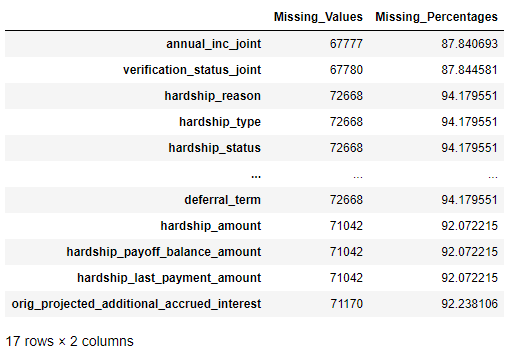
\includegraphics{MissingValues.png}
	\caption{Features having more than 60 percent missing values}
	\label{fig:MissingValues}
\end{figure}
 
\begin{table}[h!]
	\centering
	\begin{tabular}{ |p{4cm}|p{3cm}|p{3cm}|  }
		\hline
		\multicolumn{2}{|c|}{Categorical Features} \\

		\hline
		$emp\_title$ & 28185 \\
		$application\_type$ & 2 \\
		$home\_ownership$ & 5 \\
		$loan\_status$ & 7 \\
		$int\_rate$ & 129 \\
		$term$ & 2 \\
		$grade$ & 7 \\
		$earliest\_cr\_line$ & 622 \\
		$verification\_status$ & 3 \\
		$pymnt\_plan$ & 1 \\
		$purpose$ & 13 \\
		$hardship\_flag$ & 2\\
		$initial\_list\_status$ & 2\\
		$revol\_util$ & 1074 \\
		\hline
	\end{tabular}
	\caption{List of Categorical Features with unique values}
	\label{table:1}
\end{table}


\begin{figure}[h!]
	\centering
	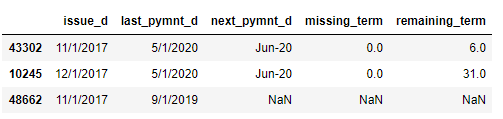
\includegraphics{dates.png}
	\caption{Transformation of Dates Columns}
	\label{fig:dates}
\end{figure}


\section{Data Preprocessing}
\subsection{Feature Engineering/Removal}
As it is discovered from figure \ref{fig:MissingValues} that we have 17 features that have more than 60 percent of null values, so we have to remove those features from the data. After removing those columns we left with 91 columns. After analysis, I found that $id$, $emp\_title$ has more than 20000 unique values so it is better to remove them from the data. $payment\_plan$ will also be dropped because it has only one unique value. In the pre-processing stage, I transformed date columns into some meaningful information like $missing\_term$, $remaining\_term$. $missing\_term$ means number of missing installments and $remaining\_term$ means duration remaining for that loan or can be interpreted as number of future installments remaining. Figure \ref{fig:dates} shows there is a pattern in these dates if we add loan term to $issue\_date$ we can get $end\_date$ and if we get the difference of $end\_date$ and $next\_pymnt\_d$ we can get $remaining\_term$. If we take difference between $next\_pymnt\_d$ and $last\_pymnt\_d$ we can calculate $missing\_term$. After creating $missing\_term$ and $remaining\_term$ I dropped the date features.

\subsection{Feature Encoding}
After some feature engineering and feature removal, I encode the categorical features. As mentioned above $int\_rate$, $revol\_util$ and $term$ is converted to continuous numeric values by removing the $\%$ symbol and $month$ from the end of each value. After this, I still left with 7 categorical columns which need encoding. Features like $application\_type$, $hardship\_flag$ and $initial\_list\_status$ has only two unique values so it is better to use OneHotEncoder and features like $home\_ownership$, $grade$, $purpose$ and $verification\_status$ has more than 2
unique values so I used OrdinalEncoder for these features. I did feature encoding before the train-test split because encoding after splitting will increase computation, I would had to do encoding separately on the test set. Encoding before the splitting does not expose our test set to the trained model. After the encoding I split the data into train-test right before the pre-processing because imputation and outlier detection might get expose our test data to models, this concept is known as Preventing data leakage in machine learning.
 
\subsection{Outlier Detection}
Outliers are the abnormal data points that may lead to bad predictions. There are number of techniques and algorithms that can be used to detect outliers. I used the IsolationForest algorithm to detect outliers. Handling with outliers needs some observation, \citep{outlier} states how to deal with outliers whether we should keep outliers or remove outliers. If we have a large number of outliers then it means outliers might present some useful information. But if the number of outliers is small as compare to total data we can drop them. In my case, I got 6000 outliers so I drop those data points from data. Before applying IsolationForest I imputed the data with zero just to make isolation forest work. Real imputation is done after the outlier handling because this will prevent bias on data.

\subsection{Imputation}
Imputation is another important step in data pre-processing because if there are missing values in the dataset and if we try to create a model with missing values, most machine learning algorithms give an error. As a result, you'll need to pick one of the imputation tactics. There are many techniques for the imputation of missing values in the dataset such as dropping the rows, imputing with nearest values, imputing with up and down values, or imputing with the mean value. For simplicity in our case, Mean-imputation is used, because imputing with mean preserves the mean of that particular feature, the estimate of the mean remains unbiased whereas for the categorical feature, I have missing values in $hardship\_flag$ I imputed with the most frequent value in this feature. Imputation on test set was done by the mean of train set features. There are benefits and disadvantages of mean imputation that are not in the scope of this project.

\subsection{Normalization}
Normalization is a data transformation method that is regularly utilized in machine learning. Normalization is the way toward changing over the upsides of numeric columns in a dataset to a comparable scale without influencing the ranges of values. Many machine learning algorithms, such as support vector machines and k means, are sensitive to normalization, although many other algorithms may function without it. Also because dimensionality reduction techniques like Principal Component Analysis (PCA) are sensitive to normalization, so I had to do normalization before dimensionality reduction.

\subsection{Feature Selection/Dimensionality Reduction}
Dimensionality reduction is a critical step in a machine learning project since characteristics that are connected to each other may produce data redundancy, which can lead to overfitting during model training. It is critical to eliminate elements that are not necessary for model training. Both the test set and the train set should have their dimensions reduced. For feature selection, a variety of methods and approaches can be applied, the comparative study on the dimensionality reduction is done by \citep{dimensionality}, however correlation threshold and principal component analysis were applied in this study. We can see which features for the model training are essential via correlation(removing the highly correlated features from data), but we only get reduced dimensioned vectors via PCA. The most used methods for dimensionality reduction are 'Projection Methods'. The goal of projection methods is to minimise the number of dimensions in the feature space while keeping the most significant structure or connections between the variables in the data. PCA is one of the projection method which can be good for feature reduction as correlation threshold might be contradictory to select. Comparison of the results obtain from PCA and correlation threshold will be discussed in the report later.


\section{Supervised Learning (Classification)}
\subsection{Target Class Transformation}
In the actual data we have seven different classes named as $fully\_paid$, $current$, $default$, $Late(15\ to\ 30\ days)$, $Late(30\ to\ 120\ days)$, $Grace\ Period$ and $Charged\ Off$ . After analysis it is concluded that $Late(15\ to\ 30\ days)$, $Late(30\ to\ 120\ days)$, $Grace\ Period$, $Charged\ Off$ and $default$ are the bad loans so I transform all these classes into a new class named as bad loan. While $fully\_paid$ remains the same as it represents that fully paid are actually good loans lastly $current$ class also remains the same as it can be either good loan or bad loan in future, so we might think these entries as loans under observation. Figure \ref{fig:new_classes} represents the distribution of target feature.
\begin{figure}[h!]
	\centering
	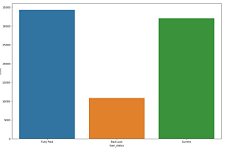
\includegraphics{classes.png}
	\caption{Transformed target feature}
	\label{fig:new_classes}
\end{figure}

\subsection{Data Balancing}
Imbalanced data occurs when the amount of observations for all of the classes in a classification dataset is not equal. Many machine learning classifiers struggle with unbalanced training datasets because they are sensitive to the ratios of various classes. As a result, these algorithms prefer the class with the highest set of observations, which might lead to inaccurate results. This can be especially problematic when we are looking for the rare class identification since many algorithms are unable to find sufficient data for learning. We can delete entries from the majority class to balance the data, but this may result in the loss of some crucial information; another option is to add duplicate values, which is also inefficient. Our data is also highly imbalance, balancing is necessary otherwise algorithm don't have enough data for minority class for learning, so for this SMOTE technique is used, SMOTE creates new records rather than duplicating the records from the dataset which is very good for highly imbalanced data. \citep{balancing} uses SMOTE for classification algorithms for highly imbalance data for comparative study so I try SMOTE for my classification problem which produces pretty good results.


\subsection{Data Splitting}
I split the data at the very beginning in the train-test set before any pre-processing starts because it prevents data leakage. Data leakage means test data might get exposed to the trained model. If I split data after the pre-processing then there are chances that my test data get expose to the trained model. I split the data into 80 20 ratios, which means a 20 percent test set and 80 percent training set. For the validation, I did cross-validation to check whether my trained model works well on unseen data or not. Although cross-validation takes a lot of processing resources so I did cross-validation only on 1 machine learning algorithm.

\subsection{Training}
The term "model training" refers to feeding data into a machine learning algorithm so that it can generate predictions. To obtain predictions, a Decision Tree, Random Forest, Adaboost are used in this study. These algorithms were used twice, the first time with features obtain from correlation threshold and the second time using principal component analysis (PCA). GridSearch is used while training these machine learning algorithms so that model gets trained with good parameters this is also known as Parameter Hyper-tuning. The results from both trials are pretty impressive, with over 80$\%$ accuracy on both the test and the train set. Table \ref{table:accuracies} shows the accuracies of the models on training set.

\begin{table}[h!]
	\centering
\begin{tabular}{ |p{3cm}|p{3cm}|p{3cm}|  }
	\hline
	\multicolumn{3}{|c|}{Train Set Results} \\
	\hline
	& Correlation Threshold & PCA \\
	\hline
	Decision Trees & 0.9397 &0.8532 \\
	Random Forest & 0.9309   & 0.8731 \\
	Adaboost &0.9224 & 0.8649 \\
	\hline
\end{tabular}
\caption{Training set accuracies with respect to feature reduction technique}
\label{table:accuracies}
\end{table}


\subsection{Testing}
In testing, we must examine our test data accuracies on trained models; in this study, I feed test data to our trained models to obtain test data predictions. Models trained using PCA provides more than 80 percent accuracy on the test set, whereas models trained with correlation threshold provide more than 90 percent accuracy on the test set. Table \ref{table:test_accuracies} shows the overall accuracy of the test sets on the trained models.
\begin{table}[h!]
	\centering
	\begin{tabular}{ |p{3cm}|p{3cm}|p{3cm}|  }
		\hline
		\multicolumn{3}{|c|}{Test Set Results} \\
		\hline
		& Correlation Threshold & PCA \\
		\hline
		Decision Trees & 0.9406 &0.8101 \\
		Random Forest & 0.9428   & 0.8396 \\
		Adaboost &0.9375 & 0.8545 \\
		\hline
	\end{tabular}
	\caption{Test set accuracies with respect to feature reduction technique}
	\label{table:test_accuracies}
\end{table}

\subsection{Classification Experiment Comparison and Evaluation}
Table \ref{table:correlation_results} and table \ref{table:pca_results} shows the experiment results and findings of different algorithms applied with different feature reduction methods. By looking at the tables it can be seen that AdaBoost works well with Principal Component Analysis and with Correlation threshold as compared to other algorithms. Adaboost is an ensemble classifier which has different variants, adaboost.M1 and adaboost.M2 that works for classification introduced by \citep{adaboost}. Other algorithms like decision tree, the random forest also has an overall accuracy of 94 percent, and recall for the minor class is just above the 60 percent with correlation threshold which is also impressive. With the PCA decision tree, the random forest has an overall accuracy of 81 percent and 84 percent, and recall for the minor class is approximately 80 percent. As our data is quite an imbalance so accuracy might not be a good measure to evaluate the model, if our recall for minority class is good then we can say that our model performs well on test data. Recall tells the percentage of correctly predicted values of a particular class so if our minority class records are correctly identified by the model then we can say that model is working well on the test data. So from table \ref{table:correlation_results} and table \ref{table:pca_results} it is concluded that Adaboost with PCA has a 0.81 recall for minority class ($bad\_loan$), and has 0.85 overall accuracy which is good among other algorithms.  
\begin{table}[h!]
	\centering
	\begin{tabular}{ |p{3cm}||p{2cm}|p{2cm}|p{2cm}|p{2cm}|  }
		\hline
		\multicolumn{5}{|c|}{Correlation Threshold Results} \\
		\hline
		& Target Class & Precision & Recall & Overall Accuracy \\
		\hline
		Adaboost & Fully Paid & 0.91 & 0.99 & 0.94\\
					  & Bad Loan & 0.95   & 0.63 & \\
					  & Current &0.96 & 0.98 & \\
		\hline
		Decision Tree & Fully Paid & 0.92 & 0.99 & 0.94\\
		& Bad Loan & 0.92 &  0.62 & \\
		& Current &0.97 & 0.99 & \\
		\hline
		Random Forest & Fully Paid & 0.92  & 1.00 & 0.94\\
		& Bad Loan & 0.98  &  0.61 & \\
		& Current & 0.96   &   1.00 & \\
		\hline
	\end{tabular}
	\caption{Correlation Results}
	\label{table:correlation_results}
\end{table}




\begin{table}[h!]
	\centering
	\begin{tabular}{ |p{3cm}||p{2cm}|p{2cm}|p{2cm}|p{2cm}|  }
		\hline
		\multicolumn{5}{|c|}{PCA Results} \\
		\hline
		& Target Class & Precision & Recall & Overall Accuracy \\
		\hline
		Adaboost & Fully Paid &0.86 & 0.88 & 0.85\\
		& Bad Loan & 0.86 & 0.81 & \\
		& Current & 0.85 & 0.84 & \\
		\hline
		Decision Tree & Fully Paid & 0.80 & 0.84 & 0.81\\
		& Bad Loan & 0.85 &  0.80 & \\
		& Current &0.81 &  0.78 & \\
		\hline
		Random Forest & Fully Paid & 0.82 & 0.88 & 0.84\\
		& Bad Loan &0.98  & 0.79 & \\
		& Current & 0.83 & 0.81 & \\
		\hline
	\end{tabular}
	\caption{PCA Results}
	\label{table:pca_results}
\end{table}

\section{Unsupervised Learning (Clustering)}
For the unsupervised learning, I took the entire data, pre-processed that data with similar techniques as I did in classification but feature reduction is done by some projection methods like PCA, FAMD. As we have high number of features we have to use projection methods before clustering, \citep{DRK} explains projection methods can be used to reduce dimensions of the data for clustering. Like classification I did some comparative study, tried to predict clusters under different scenarios. I use K-MEANS with some dimensionality reduction methods and K-Prototype which is an advance version of K-MEANS.
\subsection{Issue with data for clustering}
As our dataset contains some categorical information so applying K-MEANS directly to the data will not work because K-MEANS work by calculating the distance so K-MEAN considers our encoded categorical features as continuous numeric value but in reality, these encoded features are discrete values. To overcome this problem I use projection methods like PCA, FAMD for dimensionality reduction. Factor analysis of mixed data types (FAMD) accepts data with continuous numeric values and categorical values and produces the reduced dimensioned data. Except for K-MEANS with projection methods I also applied K-Prototype which is the latest version of KMEANS which deal with categorical features on its own, it calculates the distance differently on categorical features as compare to numerical feature.


\subsection{Elbow Scoring and Silhouette Scoring}
Elbow methods help to calculate the optimal number of clusters for the clustering algorithm. I applied the elbow method for K-MEANS after reducing the data dimensionality with PCA and FAMD. After determining the number of the optimal cluster we have to check the Silhouette score which is a matrix used to check the goodness of the clusters. Figure \ref {fig:scores} shows silhouette scores with clusters from 2 to 5 for PCA and FAMD reduced data.
%\begin{figure}[h!]
%	\centering
%	\includegraphics{pca_elbow.png}
%	\caption{Elbow method estimation for PCA reduced data}
%	\label{fig:elbow_result}
%\end{figure}
%\begin{figure}[h!]
%	\centering
%	\subfloat[\centering Elbow method estimation for FAMD reduced data %]{{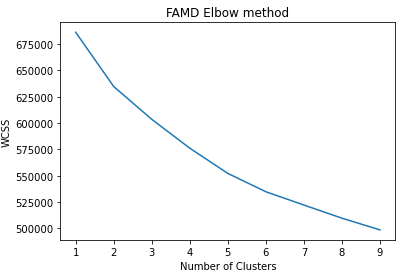
\includegraphics[width=7cm]{famd_elbow} }}%
%	\qquad
%	\subfloat[\centering Elbow method estimation for PCA reduced %data]{{\includegraphics[width=7cm]{pca_elbow} }}%
%	\caption{Elbow method estimation for FAMD and PCA Data}%
%	\label{fig:elbow_result}%
%\end{figure}

.
%\begin{figure}[h!]
%	\centering
%	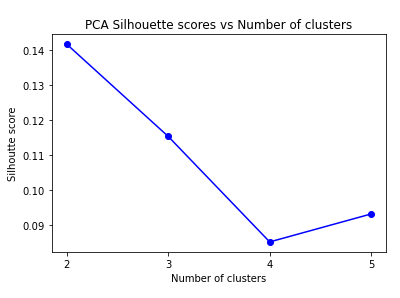
\includegraphics{pca_score.png}
%	\caption{Silhouette Scores for the PCA reduced data}
%	\label{fig:scores}
%\end{figure}
\begin{figure}[h!]
	\centering
	\subfloat[\centering Silhouette Scores for the FAMD reduced data ]{{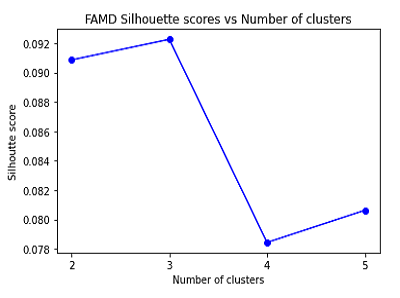
\includegraphics[width=7cm]{famd_scores} }}%
	\qquad
	\subfloat[\centering  Silhouette Scores for the PCA reduced data]{{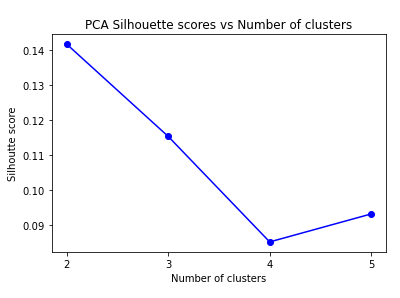
\includegraphics[width=7cm]{pca_score} }}%
	\caption{Silhouette scores for the FAMD and PCA reduced data}%
	\label{fig:scores}%
\end{figure}

 After observing figure \ref{fig:scores} it can be seen that the best optimal silhouette score is 0.14 for PCA reduced data with 2 clusters which is highest in both graphs. So for good predictions, it is better to apply K-MEANS with 2 clusters on PCA reduced data.

\subsection{K-MEANS}
After getting the data which is transformed by PCA we have no discrete values in the data and we also have the optimal number of clusters from elbow method and silhouette score, so we can apply K-MEANS. I applied K-MEANS on PCA reduced data with 2 clusters to get predictions, the results of the K-MEAN with 2 clusters are shown in figure \ref{fig:kmeans_result_2d}. By looking at figure \ref{fig:kmeans_result_2d} it can be seen that our data has a definite pattern.
\begin{figure}[h!]
	\centering
	\subfloat[\centering PCA reduced data K-MEANS clusters in 3d Scatter plot]{{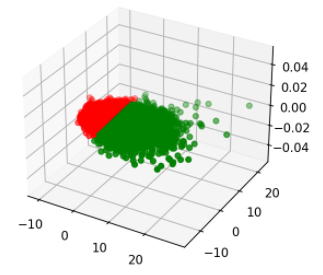
\includegraphics[width=7cm]{pca_3d} }}%
	\qquad
	\subfloat[\centering PCA reduced data K-MEANS clusters in 2d Scatter plot]{{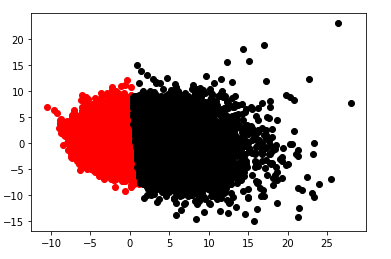
\includegraphics[width=7cm]{pca_2d} }}%
	
	\caption{K-MEANS Prediction on PCA Data}%
	\label{fig:kmeans_result_2d}%
\end{figure}

\subsection{Experiment with other algorithm}
K-Prototypes is a lesser-known version of K-MEANS that has the benefit of working with a variety of data types. In \citep{kp02} and \citep{kp01} K-Prototype algorithm is used for clustering, as problems dataset has mixed data type. It uses Euclidean distance (like K-means) to assess distance between numerical features, but it also uses the number of matching categories to evaluate distance between categorical data. I applied K-Prototype to the original data which has categorical and numerical values in it. As it has categorical values so scoring for the K-Protoype is difficult to get, it requires some mathematics, which is not in the scope of this study. I applied K-Prototype just to visualize that whether our data shows some pattern with algorithms other than K-MEANS or not. The experiment results with K-Prototype is shown in the figure \ref{fig:k_pro_re}


\begin{figure}[h!]
	\centering
	\subfloat[\centering K-Protype clusters in 3d Scatter plot]{{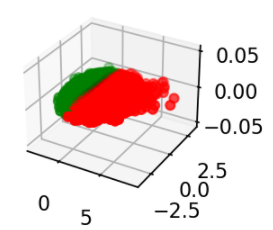
\includegraphics[width=7cm]{kp_3d} }}%
	\qquad
	\subfloat[\centering K-Prototype clusters in 2d Scatter plot]{{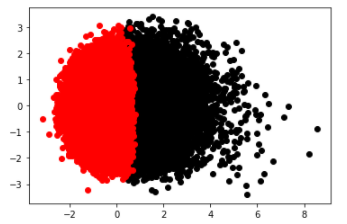
\includegraphics[width=7cm]{kp_2d} }}%
	
	\caption{K-Prototypes Predictions}%
	\label{fig:k_pro_re}%
\end{figure}

As K-Prototypes works with categorical columns so it is not possible to calculate the optimal number of clusters with silhouette score, instead optimal number can be calculated by model calculation cost. Figure \ref{fig:kp_cost} shows the optimal number of cluster with respect to the cost.
\begin{figure}[h!]
	\centering
	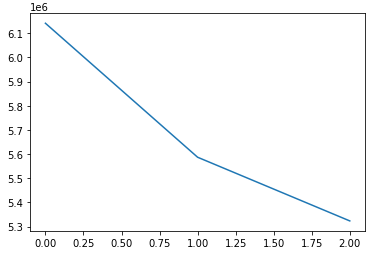
\includegraphics{kp_cost.png}
	\caption{Optimal Number of clusters with respect to cost}
	\label{fig:kp_cost}
\end{figure}

\subsection{Clustering Visualization}
As I have high-dimensionality data so we cannot plot graphs based on selected features, so we have to transform our data into 2 or 3 dimensions. For this feature reduction, I used PCA which converts my entire data into 2 or 3 vectors, after that, I used this data for visualizing against clustering model predictions.  Figure \ref{fig:kmeans_result_2d} and figure \ref{fig:k_pro_re} were created using these reduced data.
\subsection{Clustering Results}
Table \ref{table:clustering_results} shows the predictions for K-MEANS for each class. As we already know the target class so I created a matrix that tells how many records for each class are predicted in cluster 1 and cluster 2.
For $fully\_paid$ class K-MEANS predicted 22166 records for cluster 1 and 12123 for cluster 2 similarly for $bad\_loan$ class 7271 records are predicted in cluster 1 and 3560 records are predicted for cluster 2 and for the current class K-MEANS predicted 20556 in cluster 1 and 11483 in cluster 2. In the real world scenario we don't know the target class, so this interpretation is not possible.
\begin{table}[h!]
	\centering
	\begin{tabular}{ |p{2cm}|p{2cm}|p{2cm}|p{2cm}|  }
		\hline
		\multicolumn{4}{|c|}{Clustering Results} \\
		\hline
		Target Class & Total Length & Cluster 1 & Cluster 2 \\
		\hline
		 Fully Paid & 34289  & 22166 & 12123\\
		Bad Loan & 10831 & 7271 & 3560\\
		Current & 32039 & 20556 & 11483\\
		\hline
	\end{tabular}
	\caption{Clustering Results}
	\label{table:clustering_results}
\end{table}
\section{Experiment Findings}
In this study classification and clustering are performed on lending club data. In classification after using two different feature selection methods with different classification algorithms, Adaboost produces good results as compare to other algorithms with different feature selection methods. With correlation threshold feature selection method Adaboost provides overall accuracy of 0.94 and recall of 0.63 on minority class which tells that AdaBoost has really good overall accuracy but produces a bit lower recall of minority class which might be not appropriate, on the other hand, AdaBoost with PCA provides some really good results having the overall accuracy of 0.85 and recall of minority class is 0.81 which shows that PCA with Adaboost has the high accuracy of predicting minority class. Except for recall of minority class, precision and recall of all classes are approximately 0.80. From this, I concluded that as compare to the correlation threshold method for selecting features, PCA works well. For clustering, this study involves K-MEANS with PCA, FAMD, and K-Prototypes. I found that PCA gives the highest silhouette scores with 2 clusters for the K-MEAN algorithm it can be seen in the figure \ref {fig:scores}. From this, it can be concluded PCA performs better as compare to FAMD even though FAMD is for mixed data types. If we encode our categorical features and apply PCA to reduce dimensions it gives good results as compare to FAMD. As I have only 2 clusters in unsupervised learning and I have multiple classification with three classes I cannot compare results.

\section{Conclusion}
In this study, by following KDD steps I applied classification and clustering algorithm on lending club data, data is highly imbalanced and has high dimensionality. I applied Decision Tree, Random Forest, Adaboost for classification, with different feature reduction methods. It is concluded that Adaboost with PCA delivers good accuracy and recall. As data is highly imbalanced so recall is a decent matrix for assessment, AdaBoost with PCA gives over 0.80 recall which is a decent score. For the clustering, I again did some comparative study I used PCA and FAMD for dimensionality reduction. PCA with 2 clusters gives a better silhouette score. I created a matrix for clustering which tells that how many records of each class are predicted in cluster 1 and cluster 2.

\singlespacing

\bibliographystyle{agsm}
\bibliography{document}

\end{document}




